\documentclass{beamer}

\mode<presentation> {

\usetheme{default}
%\usetheme{Rochester}
%\usecolortheme{lily}

\setbeamertemplate{footline}[page number] 
\beamertemplatenavigationsymbolsempty
\setbeamertemplate{bibliography item}{} %Remove icons in bibliography
}

\usepackage{graphicx} % Allows including images
\usepackage{amsmath}
\usepackage{lmodern}
\usepackage{listings}
\usepackage{hyperref}
\usepackage{wrapfig}



\usepackage{tikz}
\usetikzlibrary{bayesnet}

\lstset{
    language=[5.0]Lua,
    basicstyle=\fontsize{11}{9},
    sensitive=true,
    breaklines=true,
    tabsize=2
}

%----------------------------------------------------------------------------------------
%	TITLE PAGE
%----------------------------------------------------------------------------------------

\title[SGVB_topic]{SGVB Topic Modelling} 

\author{Otto Fabius} 
\institute[UvA] 
{University of Amsterdam \\
Supervisor: P.Putzky \\ 
Co-Supervisors: M. Welling, D.P. Kingma
\medskip
}
\date{\today} % Date, can be changed to a custom date

\begin{document}

\begin{frame}
\titlepage % Print the title page as the first slide
\end{frame}


%----------------------------------------------------------------------------------------
%	PRESENTATION SLIDES
%----------------------------------------------------------------------------------------

\begin{frame}
\frametitle{Current Status}
\begin{itemize}
\item{Implemented LDA for baseline comparison}
\item{Implemented current version of VAE topic model}
\item{Trained a few VAE topic models on small dataset (KOS) and large dataset (NYT)}
\item{Implemented perplexity calculation as in DEF (state-of-the-art)}
\end{itemize}

\end{frame}


\begin{frame}
\frametitle{In progress}
\begin{itemize}
\item{Implementing DEF perplexity calculation method for LDA}
\item{Figuring out how to compare to DEF}
\end{frame}

\begin{frame}
\frametitle{Inference method as in DEF:}
\begin{itemize}
\item{perform inference (=get topic distribution) for 10\% of each held-out document}
\item{Calculate distribution over word probability by sampling from the topic distributon $p(w|z, \phi)$}
\end{frame}

\begin{frame}{}
\frametitle{LDA and SGVB Topic Model}
\begin{minipage}[r]{0.45\textwidth}
\centering
    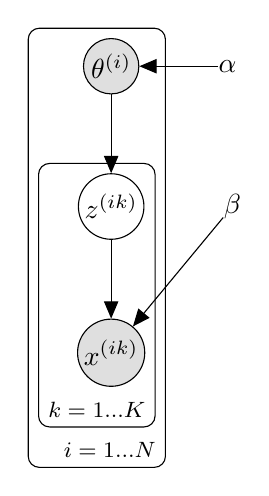
\begin{tikzpicture}[node distance = 1.5cm]
        \node[obs] (x) {$x^{(ik)}$}; 

        \node[latent, above=of x] (z) {$z^{(ik)}$}; 
        
        \node[obs, above=of z] (d) {$\theta^{(i)}$}; 

        \node[const, right=of d] (a) {$\alpha$} ;
        \node[const, right=of z] (th) {$\beta$} ;
		
		\edge {a} {d};
        \edge {z} {x};
        \edge {d} {z};
        \edge {th} {x};

		
		\plate {xz} {(x)(z)} {$k = 1...K$};
        \plate {xzd} {(x)(z)(d)(xz)} {$i = 1...N$};
	  
    \end{tikzpicture}
\end{minipage}%
\begin{minipage}{0.50\textwidth}
    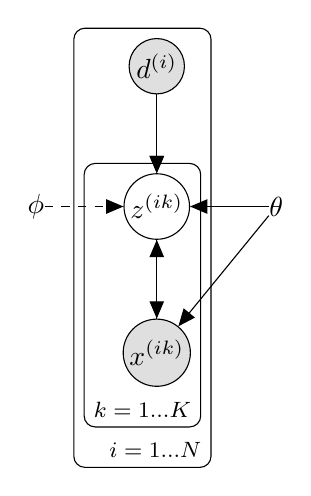
\begin{tikzpicture}[node distance = 1.5cm]
        \node[obs] (x) {$x^{(ik)}$}; 

        \node[latent, above=of x] (z) {$z^{(ik)}$}; 
        
        \node[obs, above=of z] (d) {$d^{(i)}$}; 

        \node[const, right=of z] (th) {$\theta$} ;
        \node[const, left=of z] (ph) {$\phi$};

        \edge {z} {x};
        \edge {d} {z};
        \edge {th} {z};
        \edge {th} {x};

        \edge [dashed] {ph} {z}
        \edge [dashed,bend right] {d} {z}
        \edge [dashed,bend left] {x} {z}
		
		\plate {xz} {(x)(z)} {$k = 1...K$};
        \plate {xzd} {(x)(z)(d)(xz)} {$i = 1...N$};

    \end{tikzpicture}
\end{minipage}

\vspace{5mm}

\hspace{15mm} LDA \hspace{25mm} SGVB Topic Model
\end{frame}

\begin{frame}
\frametitle{Advantages of SGVB Topic model}
Main advantage: The dependencies can be (powerful) deep nets. \\ \vspace{5mm}
This avoids the restictions of the Multinomial dependencies of LDA. The power deep learning allows it to make full use of large amounts of data.
\end{frame}

\begin{frame}
\frametitle{Preliminary Results}
\vspace{-2mm}
\begin{figure}
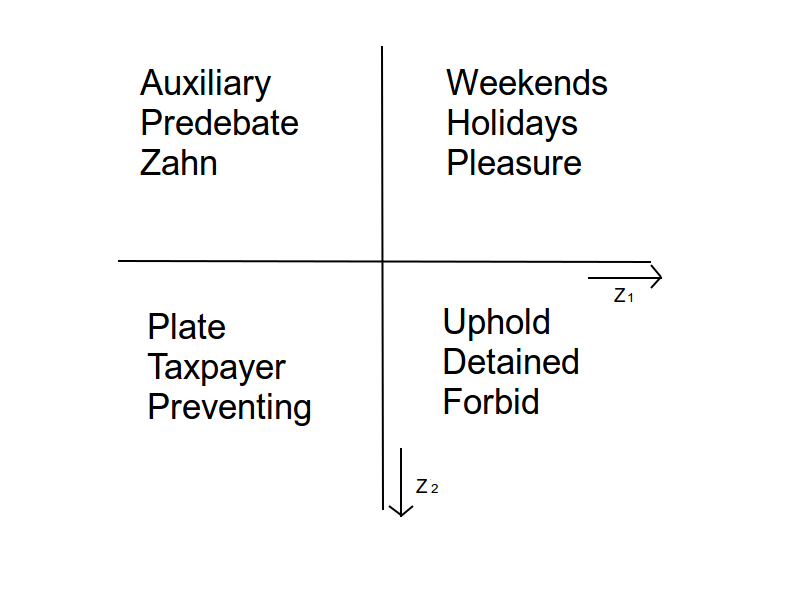
\includegraphics[scale=0.3]{superkutte_visualisatie.png}
\vspace{-12mm}
\caption{The inferred latent representation Z of documents models the topic distribution. This figure shows some frequent words for 4 regions in latent space for an SGVB Topic model with 2 latent dimensions, trained on the KOS blog posts dataset\footnote{Lichman, M. (2013). UCI Machine Learning Repository [http://archive.ics.uci.edu/ml]. Irvine, CA: University of California, School of Information and Computer Science.}}
\end{figure}
\end{frame}
\end{document}